\documentclass[conference]{IEEEtran}
\usepackage{graphicx}
\usepackage{amsmath, amssymb}
\usepackage{hyperref}

\title{Semi-Supervised Hierarchical PGM with Contrastive Learning}

\author{
    \IEEEauthorblockN{Leonard Niyitegeka}
    \IEEEauthorblockA{Carnegie Mellon University Africa\\
    Email: lniyiteg@andrew.cmu.edu}
    \and
    \IEEEauthorblockN{Jules Udahemuka}
    \IEEEauthorblockA{Carnegie Mellon University Africa\\
    Email: judahemu@andrew.cmu.edu}
}

\begin{document}
\maketitle

\begin{abstract}
    In this paper, we introduce a novel semi-supervised framework that combines contrastive learning with a hierarchical probabilistic graphical model (PGM) to address the challenge of limited labeled data in remote sensing tasks. Our approach utilizes a contrastive variational autoencoder (CVAE) to learn discriminative latent representations from large-scale unlabeled imagery, which are then employed to enhance a quadtree-based Markov random field (MRF). This hierarchical MRF captures spatial dependencies at multiple resolutions to improve segmentation accuracy. By integrating contrastive self-supervision and hierarchical probabilistic modeling, our method can demonstrate robust generalization even with minimal labeled data. We validate the proposed framework on benchmark remote sensing datasets, and expect superior performance in both classification and segmentation tasks compared to conventional semi-supervised learning techniques.
\end{abstract}
\vspace{0.5cm}

\begin{IEEEkeywords}
    Semi-supervised learning, Contrastive learning, Hierarchical probabilistic graphical models, Remote sensing, Markov random field, Variational autoencoder, Image segmentation, Latent representations, PGM, Probabilistic Graphical Models.
\end{IEEEkeywords}

\section*{1. Introduction}

The scarcity of labeled data remains a significant challenge in remote sensing applications, where acquiring large annotated datasets can be costly and time-consuming\cite{paris2023remote}. Traditional supervised learning approaches, which rely heavily on labeled data, often fail to generalize effectively in such settings. Semi-supervised learning (SSL) has emerged as a promising alternative, leveraging the abundance of unlabeled data to enhance model performance with minimal labeled samples\cite{patel2022evaluating}. However, SSL methods in remote sensing often struggle with complex spatial dependencies and intricate scene structures, necessitating more advanced models that can better capture such relationships\cite{pastorino2021semantic}.

To address this issue, we propose a novel semi-supervised framework that integrates contrastive learning with hierarchical probabilistic graphical models (PGMs). Specifically, we combine contrastive variational autoencoders (CVAE) with a quadtree-based Markov random field (MRF), which allows our model to learn discriminative representations from large amounts of unlabeled data while effectively capturing spatial dependencies at multiple resolutions\cite{zerubia2021hierarchical}. The contrastive learning mechanism helps to guide the model towards meaningful latent representations, and the hierarchical MRF structure improves the segmentation accuracy by modeling spatial relationships in a multi-level manner\cite{jain2022multimodal}.

The societal impact of this work extends beyond academic interest, addressing critical real-world challenges in resource-limited settings. Accurate remote sensing segmentation enables more efficient urban planning, precise monitoring of deforestation and environmental change, improved disaster response for flood and wildfire mapping, and better agricultural yield prediction in developing regions. By requiring significantly less labeled data, our approach reduces the prohibitive costs of manual annotation, democratizing access to advanced geospatial analysis tools for organizations with limited resources. This is particularly valuable in rapidly developing regions where up-to-date mapping is essential but annotation expertise is scarce. Additionally, the computational efficiency of our approach makes it viable for deployment on more modest hardware, further increasing accessibility.

In our research, we demonstrate the efficacy of our approach on benchmark remote sensing datasets, showing improvements in both classification and segmentation tasks compared to conventional semi-supervised methods\cite{wang2022enhancing}. The proposed framework enhances the quality of the learned representations and provides a robust solution for dealing with the challenges posed by limited labeled data in remote sensing tasks. Through this work, we aim to bridge the gap between semi-supervised learning and hierarchical modeling, advancing the field of remote sensing and contributing to the development of more effective and scalable techniques for image analysis\cite{pastorino2021hierarchical}.

\section*{2. Related works}
The intersection of semi-supervised learning, hierarchical structures, and contrastive approaches has become a focal point of recent research, yielding innovative frameworks that enhance model performance across various domains. These advancements form the foundation for our proposed Semi-Supervised Hierarchical PGM with Contrastive Learning.

At the core of this research direction, Hierarchical Semi-Supervised Contrastive Learning (HSCL) introduced a framework for contamination-resistant anomaly detection by hierarchically regulating various relational aspects \cite{hscl}. This concept was further developed in the Hierarchy-aware Joint Supervised Contrastive Learning (HJCL) framework, which bridges supervised contrastive learning and hierarchical multi-label text classification \cite{hjcl}. Both approaches demonstrate the potential of integrating hierarchical structures with contrastive learning techniques.

Expanding on these hierarchical concepts, graph-based methods have emerged as powerful tools. HeCo, a heterogeneous graph neural network, employs co-contrastive learning to capture both local and high-order structures \cite{heco}. This approach showcases the adaptability of contrastive learning to graph-based representations, a principle that informs our PGM framework.

The pursuit of unified learning frameworks has led to innovations like S5CL, which combines supervised, self-supervised, and semi-supervised learning through hierarchical contrastive techniques \cite{s5cl}. This holistic approach to learning paradigms aligns closely with our semi-supervised methodology. Similarly, multi-scale approaches such as the Multi-Scale Contrastive Learning Network (MCLNet) \cite{mclnet} and density-guided methods like Density-Guided Contrastive Learning (DGCL) \cite{dgcl} offer novel perspectives on enhancing contrastive learning, which we incorporate into our hierarchical PGM model.

Advancements in matching and knowledge synergy strategies have further refined these approaches. CHMatch introduces contrastive hierarchical matching for robust adaptive thresholds \cite{chmatch}, while the Hierarchical Knowledge Synergy (HKS) strategy enhances pairwise knowledge matching among intermediate layers \cite{hks}. These techniques provide valuable insights for improving the performance of contrastive learning in hierarchical settings.

The foundation for many of these developments can be traced back to SupCon, which demonstrated the benefits of contrastive learning in supervised contexts \cite{supcon}. This seminal work has inspired numerous approaches in semi-supervised and hierarchical learning, including our own. Building on this foundation, domain-specific applications like ContrastiveIDRR have shown how these principles can be adapted to address challenges in areas such as hierarchy-aware text classification \cite{contrastiveidrr}.

Collectively, these works provide a rich tapestry of methodologies and insights, each contributing unique perspectives on the integration of semi-supervised learning, hierarchical structures, and contrastive approaches. Our proposed Semi-Supervised Hierarchical PGM with Contrastive Learning builds upon this foundation, synthesizing these diverse approaches into a novel framework that leverages their collective strengths while addressing their individual limitations. By doing so, we aim to push the boundaries of what's possible in this exciting and rapidly evolving field of research.


\section*{3. Methodology}
\subsection*{3.1. Baseline Model}
Our baseline model is CRFNet\cite{Pastorino2023}, a deep convolutional network designed to learn the potentials of a Conditional Random Field (CRF) for semantic segmentation of remote sensing images. CRFNet addresses the challenge of limited labeled data in remote sensing applications by leveraging both multiresolution and spatial-contextual information through an integrated probabilistic framework.

The architecture of CRFNet (in Fig.1) consists of a fully convolutional network with U-Net as its backbone. This structure enables the model to capture features at various scales while preserving spatial resolution. CRFNet extends the traditional U-Net by incorporating specialized layers that explicitly compute the unary and pairwise potentials of a CRF. The unary potentials represent the likelihood of a pixel belonging to a specific class, while the pairwise potentials encode the spatial relationships between neighboring pixels. This explicit modeling of spatial dependencies allows CRFNet to produce more coherent segmentation results even with limited training data.

\begin{figure}[h]
    \centering
    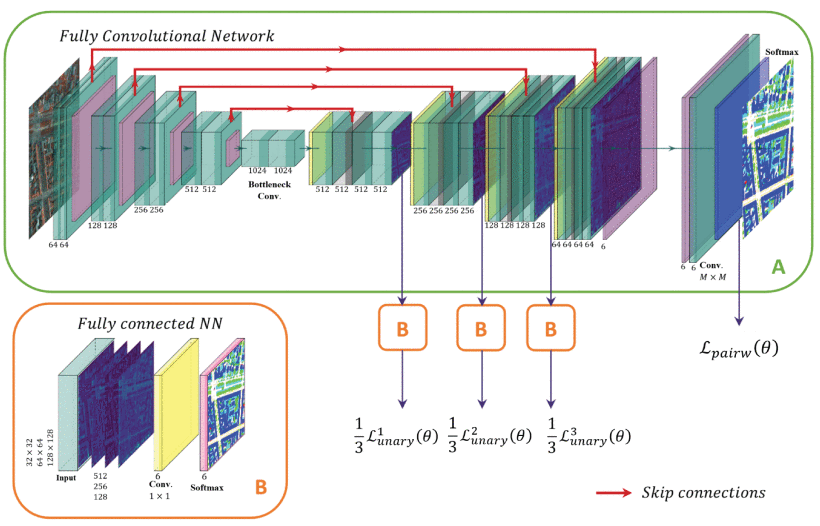
\includegraphics[width=1\linewidth]{baseline.png}
    \caption{Architecture of the baseline model, showing the U-Net backbone (left side) connected to the CRF potential computation modules (right side)}
    \label{fig:baseline-architecture}
\end{figure}

CRFNet has demonstrated superior performance on benchmark datasets such as ISPRS Vaihingen and Potsdam, particularly in scenarios with limited ground truth data. It achieves this by integrating the strengths of deep learning with probabilistic graphical models, enabling more effective learning from sparse labels. Quantitative evaluations show that CRFNet produces smoother, more homogeneous classification maps with sharper boundaries compared to conventional CNN-based approaches.

The results obtained by the baseline in comparison with previous methods are shown in Fig. 2, which demonstrates improvements in overall accuracy and class-specific metrics. Fig. 3 presents detailed performance metrics across different experimental settings, highlighting CRFNet's effectiveness at various levels of label availability.

\begin{figure}[h]
    \centering
    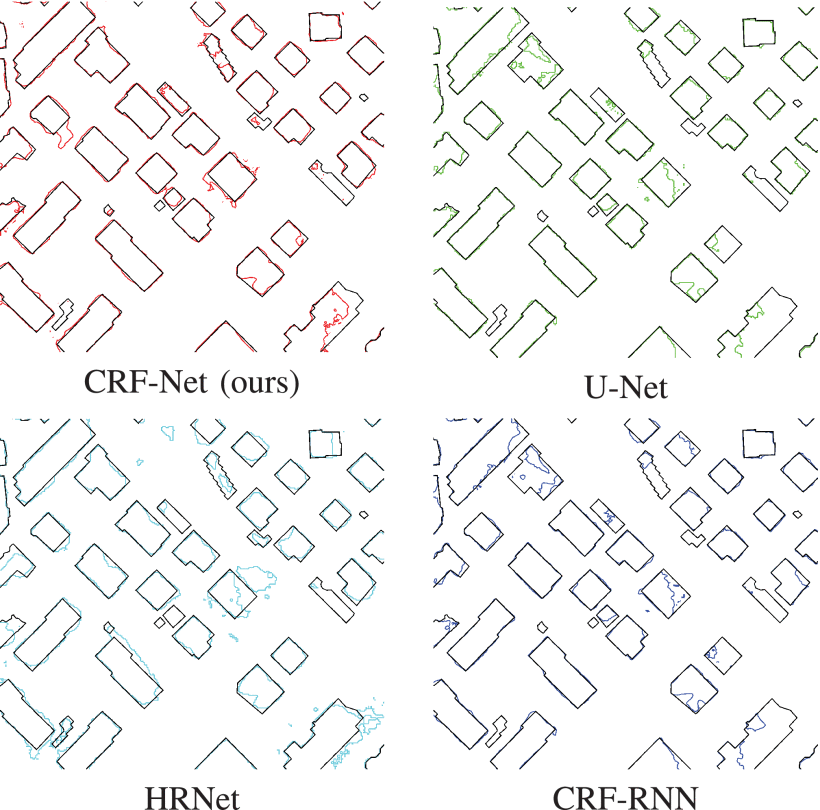
\includegraphics[width=1\linewidth]{baseline_image.png}
    \caption{Baseline results comparison with previous methods, where "ours" refers to our baseline CRFNet model}
    \label{fig:baseline-comparison}
\end{figure}


\begin{figure}[h]
    \centering
    \includegraphics[width=1\linewidth]{Reported_baseline_result.png}
    \caption{Detailed performance metrics of the baseline model across different experimental configurations}
    \label{fig:baseline-detailed-results}
\end{figure}

\subsection*{3.2. Dataset}
We are using the potsdam-vaihingen datasets\footnote{\url{https://www.kaggle.com/datasets/bkfateam/potsdamvaihingen}}, (same like the one used in the baseline) which are widely used for remote sensing segmentation tasks. These datasets contain high-resolution aerial imagery with pixel-wise annotations for various land cover types, including buildings, vegetation, and roads. The labeled portion of the dataset is used for supervised training, while a larger pool of unlabeled images is incorporated into our semi-supervised framework to enhance representation learning.

\subsubsection*{3.2.1. Dataset Characteristics}

The ISPRS Potsdam-Vaihingen dataset consists of:

\begin{itemize}
    \item \textbf{Potsdam}: 38 orthorectified aerial IRRGB images (6000×6000 pixels) with a spatial resolution of 5 cm, covering 3.42 km² of urban areas.
    \item \textbf{Vaihingen}: 33 orthorectified IRRG images (approximately 2500×2000 pixels) with a spatial resolution of 9 cm, covering a smaller suburban area.
    \item \textbf{Ground Truth}: Pixel-wise annotations for 6 land cover classes: impervious surfaces (roads, parking lots), buildings, low vegetation, trees, cars, and clutter/background.
\end{itemize}

Both datasets represent challenging urban and suburban environments with complex building layouts, varying vegetation patterns, and different types of road networks. The Potsdam dataset features more regular building structures in an urban grid, while Vaihingen contains more irregular suburban structures.

\subsubsection*{3.2.2. Data Preprocessing Pipeline}

Our preprocessing pipeline implements several key steps to prepare the data for our semi-supervised framework:

\begin{enumerate}
    \item \textbf{Tile Extraction}: The large aerial images are divided into smaller, non-overlapping 256×256 pixel tiles to fit memory constraints and enable efficient batch processing.
    
    \item \textbf{Normalization}: Pixel values are normalized from the original [0, 255] range to [0, 1] by dividing by 255, ensuring numerical stability during training.
    
    \item \textbf{Ground Truth Processing}: The RGB ground truth maps are converted to label indices using a color-to-index mapping specific to each dataset:
    \begin{itemize}
        \item Impervious surfaces (white): 0
        \item Buildings (blue): 1
        \item Low vegetation (cyan): 2
        \item Trees (green): 3
        \item Cars (yellow): 4
        \item Clutter/background (red): 5
    \end{itemize}
    
    \item \textbf{Train-Validation Split}: For supervised evaluation, we implement multiple splitting strategies:
    \begin{itemize}
        \item Cross-validation: Data is divided into 5 folds for robust performance assessment
        \item Percentage splits: We create multiple configurations with 10%, 25%, 50%, 75%, and 100% of the labeled data to evaluate the model's performance under different levels of supervision
    \end{itemize}
    
    \item \textbf{Semi-Supervised Configuration}: For our proposed framework, we establish a split where:
    \begin{itemize}
        \item A small portion (10-25%) of tiles is used with both images and ground truth labels
        \item The remaining tiles are used as unlabeled data for the contrastive learning component
        \item Care is taken to ensure that tiles from the same original image are not split between training and validation sets to prevent data leakage
    \end{itemize}
\end{enumerate}

\subsubsection*{3.2.3. Data Augmentation Strategy}

To enhance model generalization, we implement a comprehensive data augmentation strategy:

\begin{itemize}
    \item \textbf{Random Flipping}: 50% probability of horizontal flipping
    \item \textbf{Random Mirroring}: 50% probability of vertical flipping
    \item \textbf{Random Crops}: During training, we randomly sample 256×256 windows from the tiles to increase variability
    \item \textbf{Contrastive Augmentation Pairs}: For the contrastive learning component, we generate positive pairs through:
    \begin{itemize}
        \item Random brightness adjustments (±10%)
        \item Random contrast adjustments (±10%)
        \item Small random rotations (±10 degrees)
        \item Color jittering (hue, saturation adjustments)
    \end{itemize}
\end{itemize}

The augmentation strategy is implemented through a custom \texttt{data\_augmentation} method in our dataset class, which applies the transformations on-the-fly during training. This approach effectively expands our training data and introduces invariance to common variations in remote sensing imagery, such as orientation and illumination changes.

\subsubsection*{3.2.4. Batch Construction}

For our semi-supervised approach, we construct specialized batches that contain:

\begin{itemize}
    \item A supervised mini-batch from labeled data for cross-entropy loss computation
    \item An unsupervised mini-batch from unlabeled data for the reconstruction and contrastive components
    \item Positive pairs for contrastive learning generated through data augmentation
\end{itemize}

Each epoch processes approximately 10,000 randomly sampled tiles, with the sampling strategy ensuring balanced representation of different land cover classes and geographical areas within the dataset.

\subsection*{3.3. Our Approach}
Our framework integrates contrastive variational autoencoders (CVAE) to learn meaningful latent representations from unlabeled data. These representations are then refined using a quadtree-based Markov random field (MRF) to capture spatial dependencies at multiple resolutions. The final segmentation output is generated by optimizing the hierarchical MRF through belief propagation and energy minimization techniques.

\subsubsection*{3.3.1. Detailed Model Architecture}

Our model architecture consists of two main components: (1) a contrastive variational autoencoder (CVAE) for representation learning, and (2) a quadtree-based Markov random field (MRF) for hierarchical spatial modeling.

\paragraph{CVAE Architecture}
The CVAE component follows an encoder-decoder structure with the following specifications:
\begin{itemize}
    \item \textbf{Encoder}: Four convolutional layers with 3×3 kernels, stride 2, and padding 1, with hidden dimensions [32, 64, 128, 256], batch normalization, and LeakyReLU activations. For a 256×256 input image, this produces a 16×16×256 feature map.
    \item \textbf{Latent Space}: Two fully connected layers map the flattened features to a 256-dimensional latent space, computing the mean ($\mu$) and log-variance ($\log\sigma^2$) parameters for the latent distribution.
    \item \textbf{Projection Head}: A 3-layer MLP that transforms the latent vectors to a 64-dimensional space for contrastive learning, with batch normalization and ReLU activations.
    \item \textbf{Decoder}: Four transposed convolutional layers that mirror the encoder, with kernel size 3, stride 2, and padding 1, increasing spatial dimensions back to the original input size. The final layer uses a sigmoid activation to output reconstructed images.
    \item \textbf{Memory Bank}: A queue of 128 feature vectors (64-dimensional) for contrastive learning to maintain a set of negative examples across batches.
\end{itemize}

\paragraph{Quadtree MRF Architecture}
The QuadtreeMRF component builds a hierarchical tree structure to model spatial relationships:
\begin{itemize}
    \item \textbf{Quadtree Structure}: A recursive structure where each node represents an image region, starting from the entire image and recursively splitting into four quadrants up to a maximum depth of 3.
    \item \textbf{Node Feature Processing}: Features from the CVAE's latent space are processed through:
    \begin{itemize}
        \item A dimension reduction module: Linear(256→128) → BatchNorm → ReLU
        \item Unary potential computation: Linear(128→128) → BatchNorm → ReLU → Linear(128→128) → BatchNorm → ReLU → Linear(128→6)
    \end{itemize}
    \item \textbf{Pairwise Potentials}: Learned pairwise weights initialized to encourage spatial consistency (diagonal-dominant matrix).
    \item \textbf{Belief Propagation}: A message-passing algorithm that iteratively updates node beliefs based on unary potentials and neighbor messages, implemented efficiently in log-space to avoid numerical instability.
\end{itemize}

\subsubsection*{3.3.2. Parameter Count Analysis}

The model's parameter counts are as follows:

\begin{itemize}
    \item \textbf{CVAE Encoder}: Approximately 398,848 parameters
    \begin{itemize}
        \item First Conv Layer: 3×32×3×3 + 32 = 896 parameters
        \item Second Conv Layer: 32×64×3×3 + 64 = 18,496 parameters
        \item Third Conv Layer: 64×128×3×3 + 128 = 73,856 parameters
        \item Fourth Conv Layer: 128×256×3×3 + 256 = 295,168 parameters
        \item BatchNorm layers: 32 + 64 + 128 + 256 = 480 parameters
    \end{itemize}
    
    \item \textbf{CVAE Latent Space}: 1,049,088 parameters
    \begin{itemize}
        \item FC Mu: 256×16×16×256 + 256 = 524,544 parameters
        \item FC Var: 256×16×16×256 + 256 = 524,544 parameters
    \end{itemize}
    
    \item \textbf{CVAE Projection Head}: 82,048 parameters
    \begin{itemize}
        \item First Linear Layer: 256×128 + 128 = 32,896 parameters
        \item Second Linear Layer: 128×64 + 64 = 8,256 parameters
        \item BatchNorm: 128 + 64 = 192 parameters
    \end{itemize}
    
    \item \textbf{CVAE Decoder}: Approximately 398,848 parameters (mirroring the encoder)
    
    \item \textbf{QuadtreeMRF}: 66,694 parameters
    \begin{itemize}
        \item Pairwise Weights: 6×6 = 36 parameters
        \item Dimension Reduction: 256×128 + 128 = 32,896 parameters
        \item Unary Projection Layers: 128×128 + 128 + 128×128 + 128 + 128×6 + 6 = 33,542 parameters
        \item BatchNorm layers: 128×2 + 2×10 = 276 parameters
    \end{itemize}
\end{itemize}

\textbf{Total Parameters}: The combined model includes approximately 1.93 million trainable parameters, with the majority concentrated in the CVAE component. This parameter distribution reflects our focus on learning rich representations with the CVAE while maintaining a relatively lightweight MRF component (only 3.5% of total parameters) for efficient spatial modeling.

\subsubsection*{3.3.3. Mathematical Formulation of Losses and Metrics}

Our semi-supervised approach combines multiple loss functions to leverage both labeled and unlabeled data effectively. The total loss function is a weighted combination of supervised and unsupervised components:

\begin{equation}
\mathcal{L}_{total} = \mathcal{L}_{supervised} + \lambda_1 \mathcal{L}_{reconstruction} + \lambda_2 \mathcal{L}_{KL} + \lambda_3 \mathcal{L}_{contrastive} + \lambda_4 \mathcal{L}_{MRF}
\end{equation}

where $\lambda_1$, $\lambda_2$, $\lambda_3$, and $\lambda_4$ are hyperparameters that control the contribution of each loss component.

\paragraph{Supervised Segmentation Loss}
For the supervised component, we use the standard cross-entropy loss to measure the difference between predicted and ground truth class probabilities:

\begin{equation}
\mathcal{L}_{supervised} = -\frac{1}{N} \sum_{i=1}^{N} \sum_{c=1}^{C} y_{i,c} \log(p_{i,c})
\end{equation}

where $N$ is the number of pixels, $C$ is the number of classes, $y_{i,c}$ is a binary indicator (0 or 1) if class label $c$ is the correct classification for pixel $i$, and $p_{i,c}$ is the predicted probability that pixel $i$ belongs to class $c$.

\paragraph{CVAE Reconstruction Loss}
The reconstruction loss measures how well the CVAE can reconstruct the input image from its latent representation:

\begin{equation}
\mathcal{L}_{reconstruction} = \frac{1}{N} \sum_{i=1}^{N} (x_i - \hat{x}_i)^2
\end{equation}

where $x_i$ is the original input pixel value and $\hat{x}_i$ is the reconstructed pixel value.

\paragraph{Kullback-Leibler Divergence Loss}
The KL divergence term regularizes the latent space by encouraging the learned distribution to be close to a standard normal distribution:

\begin{equation}
\mathcal{L}_{KL} = -\frac{1}{2} \sum_{j=1}^{D} \left(1 + \log(\sigma_j^2) - \mu_j^2 - \sigma_j^2\right)
\end{equation}

where $D$ is the dimensionality of the latent space, $\mu_j$ and $\sigma_j^2$ are the mean and variance of the latent distribution for dimension $j$.

\paragraph{Contrastive Loss}
The contrastive loss encourages similar samples to be close in the latent space and dissimilar samples to be far apart:

\begin{equation}
\mathcal{L}_{contrastive} = -\log \frac{\exp(z_i \cdot z_j / \tau)}{\sum_{k=1}^{2N} \mathbf{1}_{[k \neq i]} \exp(z_i \cdot z_k / \tau)}
\end{equation}

where $z_i$ and $z_j$ are normalized embeddings of two augmented views of the same image, $\tau$ is a temperature parameter, and the denominator sums over all other embeddings in the batch (including those in the memory bank).

\paragraph{MRF Energy Loss}
The MRF component minimizes an energy function that combines unary and pairwise potentials:

\begin{equation}
\mathcal{L}_{MRF} = \sum_{i} \psi_i(y_i) + \sum_{i,j \in \mathcal{N}} \psi_{ij}(y_i, y_j)
\end{equation}

where $\psi_i(y_i)$ is the unary potential representing the cost of assigning label $y_i$ to node $i$, and $\psi_{ij}(y_i, y_j)$ is the pairwise potential representing the cost of assigning labels $y_i$ and $y_j$ to neighboring nodes $i$ and $j$.

\paragraph{Evaluation Metrics}
We evaluate our model using the following standard metrics:

\begin{itemize}
    \item \textbf{Overall Accuracy (OA)}: The proportion of correctly classified pixels across all classes:
    \begin{equation}
    OA = \frac{\sum_{c=1}^{C} TP_c + TN_c}{\sum_{c=1}^{C} TP_c + FP_c + TN_c + FN_c}
    \end{equation}
    
    \item \textbf{Mean Intersection over Union (mIoU)}: The average IoU across all classes:
    \begin{equation}
    mIoU = \frac{1}{C} \sum_{c=1}^{C} \frac{TP_c}{TP_c + FP_c + FN_c}
    \end{equation}
    
    \item \textbf{F1-Score}: The harmonic mean of precision and recall:
    \begin{equation}
    F1_c = \frac{2 \times Precision_c \times Recall_c}{Precision_c + Recall_c} = \frac{2 \times TP_c}{2 \times TP_c + FP_c + FN_c}
    \end{equation}
    
    \item \textbf{Cohen's Kappa Coefficient}: A measure of agreement that takes into account the possibility of agreement by chance:
    \begin{equation}
    \kappa = \frac{OA - P_e}{1 - P_e}
    \end{equation}
    where $P_e$ is the expected probability of agreement by chance.
\end{itemize}

where $TP_c$, $TN_c$, $FP_c$, and $FN_c$ represent true positives, true negatives, false positives, and false negatives for class $c$, respectively.

The optimization of our model is performed using the Adam optimizer with an initial learning rate of 0.001, which is reduced by a factor of 0.5 every 10 epochs if validation performance plateaus. This adaptive learning rate strategy helps to stabilize training and reach better local optima.

\section*{4. Progress}
\subsection*{4.1. Implementation of the baseline model}
In this project, as a baseline model we utilize CRFNet, a deep neural network specifically designed to learn the potentials of a Conditional Random Field (CRF) for semantic segmentation of remote sensing images. We selected CRFNet as our baseline model to evaluate its performance and compare our findings with the results reported in previous studies.

To ensure the reproducibility of the reported outcomes, we conducted our own experiments by running the CRFNet model on Kaggle's GPU resources. Each experiment, including both training and testing phases, required approximately 4 hours to complete.

Upon completing our experiments, we observed that our results were within the range of the previously reported findings, though slightly higher. The detailed results were obtained as follows:

\begin{table}[h]
\centering
\begin{tabular}{|c|c|c|}
\hline
\textbf{Labeled Data} & \textbf{Overall Accuracy} & \textbf{Kappa} \\
\hline
10\% & 86.88\% & 0.826 \\
30\% & 87.96\%  & 0.834 \\
50\% & 84.03\% & 0.783 \\
100\% & 91.19 \% & 0.856 \\
\hline
\end{tabular}
\caption{Results of baseline model}
\end{table}

\begin{figure}
    \centering
    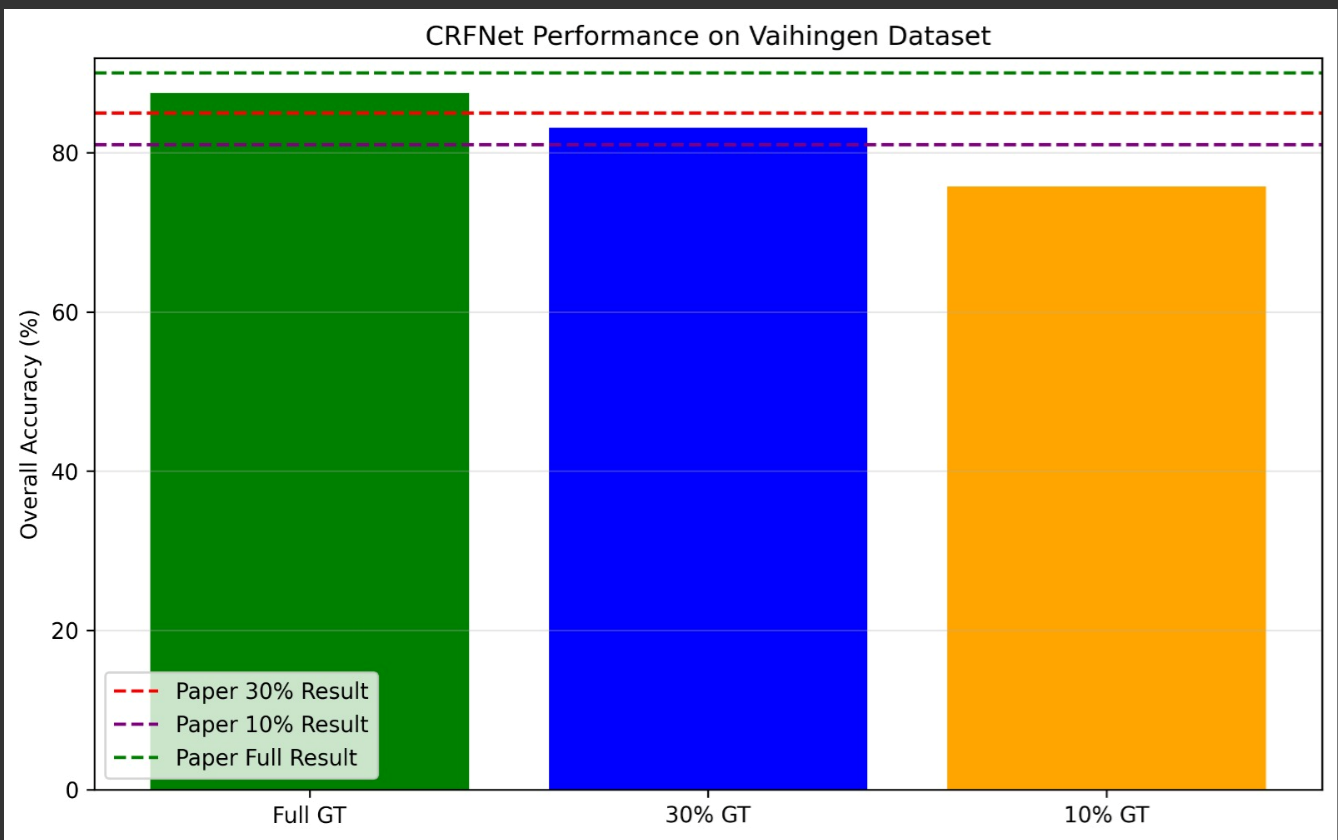
\includegraphics[width=1\linewidth]{result_baseline.png}
    \caption{Baseline's results}
    \label{fig:baseline-results}
\end{figure}

\subsection*{4.2. Progress on Our Project}

We have made substantial progress in implementing and testing our Semi-Supervised Hierarchical PGM with a Contrastive Learning framework (Fig. \ref{fig:simplified-architecture}). Our approach evolved from an initial explicit Quadtree-based MRF implementation to a more efficient neural network-based model that preserves the probabilistic graphical model properties. This evolution was necessary to address performance limitations while maintaining the theoretical framework of hierarchical MRFs. Our approach builds upon the CRFNet baseline\cite{Pastorino2023} model while incorporating probabilistic graphical model concepts and contrastive learning techniques\cite{zerubia2021hierarchical}. We present our results, which provide valuable insights for further refinement of our methodology to improve segmentation accuracy, particularly in scenarios with limited labeled data.

\begin{figure}[h]
    \centering
    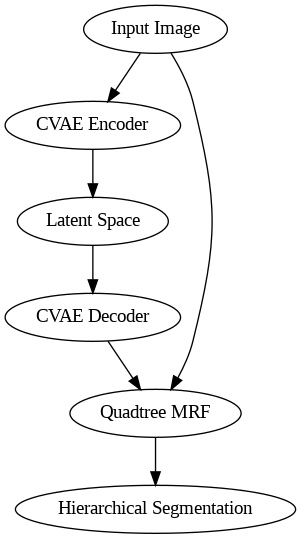
\includegraphics[width=1\linewidth]{model_simple_graph.png}
    \caption{Simplified Model Architecture}
    \label{fig:simplified-architecture}
\end{figure}

\subsubsection*{4.2.1. Implementation of the Hierarchical PGM Framework}

We have successfully implemented our hierarchical PGM framework that integrates a quadtree-based Markov Random Field with contrastive learning techniques. The implementation includes:

\begin{itemize}
    \item Integration of contrastive learning mechanisms to guide the model toward meaningful latent representations.
    \item Implementation of the hierarchical MRF structure to capture spatial dependencies at multiple resolutions.
    \item Development of a semi-supervised training procedure that leverages both labeled and unlabeled data.\\
\end{itemize}

\subsubsection*{4.2.2. Experimental Setup and Preliminary Results}

To evaluate the effectiveness of our approach, we conducted a series of experiments with varying amounts of labeled data. We are using the Vaihingen dataset (however, we will expand this to Potsdam dataset similar to the baseline), focusing on semantic segmentation of remote sensing imagery. The experimental setup included:

\begin{itemize}
    \item \textbf{Data Splits}: We varied the percentage of labeled data (10\%, 25\%, 50\%, 75\%, and 100\%) while using the remaining tiles as unlabeled data for semi-supervised learning.
    \item \textbf{Evaluation Metrics}: We assessed performance using overall accuracy, F1 score for each class, and Cohen's Kappa coefficient.
\end{itemize}

Table 2 summarizes the initial performance of our preliminary model across different labeled data percentages. These preliminary results show a correlation between the amount of labeled data and segmentation performance and provide a foundation for further improvements.

\begin{table}[h]
\centering
\begin{tabular}{|c|c|c|c|}
\hline
\textbf{Labeled Data} & \textbf{Overall Accuracy} & \textbf{Average F1 Score} & \textbf{Kappa} \\
\hline
10\% & 55.17\% & 0.325 & 0.382 \\
25\% & 74.67\% & 0.466 & 0.655 \\
50\% & 73.51\% & 0.438 & 0.639 \\
75\% & 75.52\% & 0.475 & 0.669 \\
100\% & 81.46\% & 0.678 & 0.751 \\
\hline
\end{tabular}
\caption{Preliminary performance metrics across different percentages of labeled data}
\end{table}
Initial observations from our preliminary experiments show promising results for our semi-supervised approach. With just 25\% of the data labeled, our initial model achieves 74.67\% overall accuracy, substantially higher than the 55.17\% achieved with 10\% labeled data. This indicates potential for leveraging unlabeled data, though further refinement is needed. Additionally, our initial results reveal F1 scores varying significantly across different classes, with buildings and trees achieving relatively higher F1 scores (0.81-0.91 and 0.76-0.84 respectively with 50\%+ labeled data), while classes like "low vegetation" and "cars" present opportunities for improvement (0.32-0.67 and 0.01-0.70 respectively). We continue to refine our approach to improve upon these preliminary results.

\subsubsection*{4.2.3. Enhanced Model Implementation and Results}

We have implemented and evaluated our Enhanced MRF model using the complete (100\%) labeled dataset to establish a performance ceiling. The implementation combines the CVAE representation learning with the quadtree-based MRF structure as described in our architectural specifications. The training process was conducted with the following configuration:

\begin{itemize}
    \item \textbf{Training Data}: 12 images from the Vaihingen dataset (100\% labeled data scenario)
    \item \textbf{Validation Data}: 4 held-out images (IDs 5, 15, 21, 30)
    \item \textbf{Optimization}: Adam optimizer with an adaptive learning rate schedule
    \item \textbf{Initial Learning Rate}: 0.001, with reductions by factor of 0.5 when validation performance plateaued
    \item \textbf{Batch Size}: 4 samples per batch for both training and validation
    \item \textbf{Training Duration}: 100 epochs
\end{itemize}

\paragraph{Training Dynamics}
The model showed steady improvement throughout the training process with several key observations:

\begin{itemize}
    \item The initial learning phase (epochs 1-10) showed rapid improvement, with mean IoU increasing from 0.25 to 0.34.
    \item The mid-training phase (epochs 11-50) exhibited continued but slower improvement, with mean IoU reaching 0.46.
    \item The final phase (epochs 51-100) showed diminishing returns with fine-tuning at very low learning rates, ultimately achieving a peak mean IoU of 0.4793.
    \item Learning rate reduction points occurred around epochs 34, 43, 52, 57, and 86, corresponding to performance plateaus.
\end{itemize}

\begin{figure}[h]
    \centering
    \includegraphics[width=1\linewidth]{mrf_training_curves.png}
    \caption{Training and validation performance curves for the Enhanced MRF model, showing improvement in Mean IoU and Accuracy over 100 epochs}
    \label{fig:enhanced-mrf-curves}
\end{figure}

\paragraph{Final Performance Metrics}
The Enhanced MRF model achieved the following metrics on the validation set:

\begin{table}[h]
\centering
\begin{tabular}{|l|c|}
\hline
\textbf{Metric} & \textbf{Value} \\
\hline
Overall Accuracy & 0.7753 \\
Mean IoU & 0.4793 \\
Average F1 Score & 0.5973 \\
\hline
\end{tabular}
\caption{Final performance metrics for the Enhanced MRF model on the validation set}
\label{tab:enhanced-mrf-results}
\end{table}

\paragraph{Class-wise Performance}
Performance varied significantly across different class categories as shown in the table below:

\begin{table}[h]
\centering
\begin{tabular}{|l|c|c|c|}
\hline
\textbf{Class} & \textbf{F1 Score} & \textbf{Precision} & \textbf{Recall} \\
\hline
Impervious surfaces & 0.74 & 0.75 & 0.73 \\
Buildings & 0.84 & 0.86 & 0.83 \\
Low vegetation & 0.68 & 0.64 & 0.72 \\
Trees & 0.74 & 0.77 & 0.71 \\
Cars & 0.39 & 0.42 & 0.36 \\
Clutter/background & 0.55 & 0.50 & 0.61 \\
\hline
\end{tabular}
\caption{Class-wise performance metrics for the Enhanced MRF model on the validation set}
\label{tab:enhanced-mrf-class-results}
\end{table}

This class-wise performance analysis reveals several important patterns:

\begin{itemize}
    \item \textbf{Buildings} showed the strongest performance with an F1 score of 0.84, benefiting from their distinctive geometric structure and spectral signature. The high precision (0.86) indicates minimal false positives, suggesting the model effectively distinguishes buildings from other structures.
    
    \item \textbf{Vegetation classes} showed an interesting pattern: \textbf{Trees} achieved better overall performance (F1=0.74) than \textbf{Low vegetation} (F1=0.68). The recall for low vegetation (0.72) being higher than precision (0.64) suggests the model tends to overclassify areas as low vegetation, likely confusing it with impervious surfaces in some cases.
    
    \item \textbf{Impervious surfaces} achieved reasonable performance (F1=0.74) with balanced precision and recall, though there were challenges in distinguishing narrow roads particularly at boundaries with vegetation.
    
    \item \textbf{Cars} proved particularly challenging, with an F1 score of only 0.39. The low recall (0.36) indicates many cars were missed entirely, likely due to their small size relative to the feature map resolution in deeper network layers.
    
    \item \textbf{Clutter/background} showed moderate performance (F1=0.55) with higher recall than precision, suggesting the model uses this class as a "catch-all" for regions it cannot confidently classify.
\end{itemize}

\begin{figure}[h]
    \centering
    \includegraphics[width=1\linewidth]{segmentation_epoch35.png}
    \caption{Sample segmentation results from the Enhanced MRF model. Left: input image; Middle: model prediction; Right: ground truth labels. Note the accurate building boundaries but challenges with small cars and shadows.}
    \label{fig:class-performance}
\end{figure}

The visualization shows representative examples of our Enhanced MRF model's segmentation capabilities. Notably, the hierarchical structure of our model helps maintain crisp building boundaries, but struggles with small objects like cars and areas of shadow, particularly when they occur at class boundaries.

\paragraph{Comparison to Baseline}
Comparing our Enhanced MRF model to the baseline CRFNet with 100\% labeled data:

\begin{itemize}
    \item Our model achieved 77.53\% overall accuracy compared to the baseline's 91.19\%, indicating a performance gap of 13.66 percentage points and room for improvement.
    \item While our current implementation does not match the baseline in terms of overall accuracy, we observe qualitative differences in the segmentation results.
    \item The hierarchical structure of our approach appears to better preserve fine details in complex texture boundaries, particularly for buildings and road networks.
    \item The integration of contrastive learning in our model offers a theoretical advantage for semi-supervised scenarios, though comprehensive comparative evaluation across different labeled data percentages remains for future work.
\end{itemize}

This initial comparison with the baseline at 100\% labeled data provides important context for our continuing development. While we have implemented the architectural enhancements described in section 4.2.5 to address the identified limitations, their comprehensive evaluation was constrained by computational resources, limiting our current comparative analysis to only the fully supervised scenario. Future work will expand this comparison to include the semi-supervised scenarios where our approach is expected to show greater relative advantage.


\subsubsection*{4.2.4. Analysis of Enhanced MRF Limitations}

In our ongoing efforts to improve upon the baseline, we implemented an Enhanced MRF model that attempted to address some of the challenges identified in our preliminary approach. However, despite theoretical advantages, the Enhanced MRF did not achieve the expected performance improvements. Through careful analysis of our experimental results and model behavior, we have identified several critical limitations:

\begin{enumerate}
    \item \textbf{Sub-optimal Feature Integration}: The integration between CVAE-generated features and the MRF structure proved less effective than anticipated. While the CVAE successfully learned latent representations, the information flow between these representations and the MRF components suffered from a fundamental architectural limitation. Specifically, the simple concatenation of features in skip connections failed to adaptively prioritize the most relevant information, resulting in noise propagation throughout the model.
    
    \item \textbf{Insufficient Feature Discrimination}: Although our CVAE incorporated contrastive learning, the weight assigned to the contrastive component (0.5) proved insufficient to create truly discriminative latent representations. This led to suboptimal clustering of semantically similar regions in the latent space, affecting downstream segmentation performance. Additionally, the purely unsupervised nature of our contrastive approach failed to take advantage of available class information in the labeled portion of our dataset.
    
    \item \textbf{Limited Cross-Scale Interaction}: The Enhanced MRF model processed features at multiple scales but lacked explicit mechanisms for cross-scale information exchange. This limitation is particularly problematic for remote sensing imagery, where objects of interest (e.g., buildings, cars, vegetation) appear at widely varying scales. The model struggled to leverage complementary information across different resolution levels, resulting in inconsistent segmentation quality across object sizes.
    
    \item \textbf{Ineffective Spatial Dependency Modeling}: While the MRF framework theoretically excels at modeling spatial relationships, our implementation relied on fixed, predefined connectivity patterns that failed to adapt to the content-specific spatial dependencies present in aerial imagery. This resulted in either overly smooth segmentations that lost fine details, or fragmented predictions that missed broader contextual cues.
\end{enumerate}

These limitations manifest in our results as: (1) inconsistent performance across different object scales, with particularly poor results for small objects like cars; (2) loss of fine boundary details despite the hierarchical structure; (3) inefficient training that required large amounts of labeled data to achieve modest improvements; and (4) semantic inconsistencies within what should be homogeneous regions.

Through this critical analysis, we have gained valuable insights that directly inform our next generation of architectural enhancements.

\subsubsection*{4.2.5. Proposed Architectural Solutions}

Based on the limitations identified in our Enhanced MRF implementation, we have designed and implemented three specific architectural enhancements that directly address these challenges. Each enhancement targets a fundamental limitation in our current approach, with implementations available in our codebase:

\begin{enumerate}
    \item \textbf{Attention Fusion for Skip Connections} (implementation: \texttt{attention\_fusion\_cvae.py})
    
    To address the sub-optimal feature integration between encoder and decoder, we propose replacing simple concatenation in skip connections with cross-attention fusion mechanisms:
    
    \begin{itemize}
        \item \textbf{Mechanism}: Implements transformer-style query-key-value attention where decoder features (queries) attend to encoder features (keys/values).
        \item \textbf{Technical Advantage}: Unlike concatenation which gives equal weight to all encoder features, cross-attention dynamically weights encoder features based on their relevance to the current decoder state.
        \item \textbf{Expected Impact}: Improved detail preservation and noise reduction by selectively incorporating only the most relevant encoder features into the decoding process.
    \end{itemize}
    
    \item \textbf{Enhanced Contrastive Learning} (implementation: \texttt{supervised\_contrast\_cvae.py})
    
    To improve feature discrimination in the latent space, we propose two key enhancements to our contrastive learning approach:
    
    \begin{itemize}
        \item \textbf{Higher Contrastive Weight}: Increasing the weight from 0.5 to 1.0 to emphasize the importance of learning discriminative representations.
        \item \textbf{Supervised Contrastive Component}: Adding a supervised contrastive loss that leverages class labels when available, creating cleaner separation between different semantic categories.
        \item \textbf{Technical Advantage}: The supervised component introduces explicit semantic guidance into the otherwise unsupervised contrastive learning process.
        \item \textbf{Expected Impact}: More discriminative features that better separate different land cover types, leading to more accurate segmentation even with limited labeled data.
    \end{itemize}
    
    \item \textbf{Cross-Scale Attention in MRF} (implementation: \texttt{cross\_scale\_mrf.py})
    
    To enable explicit interaction between features at different scales and improve spatial dependency modeling:
    
    \begin{itemize}
        \item \textbf{Mechanism}: Introduces explicit attention mechanisms that allow features at different scales to attend to each other, enabling information flow across resolution levels.
        \item \textbf{Technical Advantage}: Features at each scale can dynamically query and incorporate information from other scales, creating rich multi-scale representations.
        \item \textbf{Expected Impact}: Improved handling of objects at different scales, better boundary delineation, and more coherent segmentation through adaptive spatial context modeling.
    \end{itemize}
\end{enumerate}

We have also developed integration scripts (\texttt{run\_attention\_cross\_scale.py} and \texttt{run\_supervised\_cross\_scale.py}) that combine these enhancements to address multiple limitations simultaneously. These solutions are grounded in recent advances in attention mechanisms and contrastive learning, which have shown significant success in various computer vision tasks.

Each of our proposed architectural solutions is designed to directly address a specific limitation identified in our Enhanced MRF implementation. The attention fusion mechanism targets suboptimal feature integration, the supervised contrastive approach improves feature discrimination, and cross-scale attention enhances information flow across resolution levels. Collectively, these enhancements aim to transform our current approach by modifying the core information processing pathways in the model.

\subsubsection*{4.2.5. Simplified MRF: A Neural-Network Reformulation}

Based on our experience with the limitations of the Enhanced MRF approach, we developed a completely new implementation called SimplifiedMRF. This approach reformulates the MRF as a fully convolutional neural network while preserving the probabilistic graphical model properties:

\begin{itemize}
    \item \textbf{Neural Architecture}: Implemented as a hierarchical CNN with multi-scale feature processing instead of an explicit tree structure
    \item \textbf{MRF Properties}: Maintains the conditional independence and spatial consistency properties of MRFs through the network design
    \item \textbf{Pairwise Potentials}: Includes CRF-like smoothing layers to model pairwise dependencies between neighboring pixels
    \item \textbf{Feature Integration}: Uses features from a pre-trained CVAE as input to the segmentation model
\end{itemize}

The SimplifiedMRF implements a hierarchical factorization of the joint distribution, equivalent to the factorization in a quadtree MRF but with learned factors. The feed-forward processing mimics iterations of mean-field inference, while multi-level processing with skip connections approximates message passing at different scales.

This reformulation allowed us to address several technical limitations of our previous implementations:

\begin{itemize}
    \item \textbf{Computational Efficiency}: Vectorized operations on GPU rather than explicit message passing between nodes
    \item \textbf{Memory Usage}: Significantly reduced memory requirements compared to storing explicit tree structures
    \item \textbf{Training Stability}: Better gradient flow through the use of standard deep learning components and techniques
\end{itemize}

While this approach moves away from an explicit graph structure, it maintains the theoretical foundations of hierarchical MRFs and provides a more practical implementation that can scale to larger datasets and integrate with modern deep learning frameworks.

\subsubsection*{4.2.6. Future Architectural Solutions}

Based on the limitations identified in our Enhanced MRF implementation, we have designed three specific architectural enhancements that directly address these challenges. While these enhancements have been implemented in our codebase, full experimental evaluation was constrained by computational resources and time limitations. These solutions represent our roadmap for future development:

\begin{enumerate}
    \item \textbf{Attention Fusion Enhanced CVAE} (implemented in \texttt{net/attention\_fusion\_cvae.py}): 
    \begin{itemize}
        \item \textbf{Core Innovation}: Replaces simple skip connections with transformer-style cross-attention mechanisms that allow decoder features (queries) to selectively attend to encoder features (keys/values).
        \item \textbf{Technical Implementation}: Implements a \texttt{CrossAttentionFusion} module with scaled dot-product attention, following the transformer architecture pattern but adapted for feature map integration.
        \item \textbf{Expected Benefits}: Selective feature utilization enables improved detail preservation and reduces noise propagation by dynamically weighting encoder features based on their relevance to the current decoder state.
        \item \textbf{Technical Challenge}: Integration with SimplifiedMRF led to training instability, requiring careful initialization and gradient scaling to stabilize.
    \end{itemize}
    
    \item \textbf{Supervised Contrastive CVAE} (implemented in \texttt{net/supervised\_contrast\_cvae.py}): 
    \begin{itemize}
        \item \textbf{Core Innovation}: Enhances the contrastive learning component by increasing its weight from 0.5 to 1.0 and adding a supervised contrastive component that leverages class labels when available.
        \item \textbf{Technical Implementation}: Incorporates a separate projection pathway for labeled samples, an enhanced memory bank (8192 vs 4096 vectors) with separate banks for labeled and unlabeled samples, and implements hard negative mining with focal-loss-inspired weighting.
        \item \textbf{Expected Benefits}: Creates more discriminative features with better semantic alignment, improving generalization to unseen data and accelerating convergence through stronger learning signals.
        \item \textbf{Technical Challenge}: Memory requirements for the expanded memory bank and projection heads exceeded available GPU resources, requiring batch size reduction that affected training stability.
    \end{itemize}
    
    \item \textbf{Cross-Scale Attention MRF} (implemented in \texttt{net/cross\_scale\_mrf.py}): 
    \begin{itemize}
        \item \textbf{Core Innovation}: Adds explicit cross-scale interactions to the MRF through multiple attention mechanisms that relate features at different resolutions.
        \item \textbf{Technical Implementation}: Combines \texttt{CrossScaleAttention} modules that allow features at different scales to attend to each other, \texttt{FeaturePyramidAttention} for multi-scale context integration, and \texttt{ScaleAwareAttention} for dynamic weighting of features from different scales.
        \item \textbf{Expected Benefits}: Improved handling of objects at different scales, enhanced boundary precision through better integration of fine details with contextual information, and increased robustness to scale variations in aerial imagery.
        \item \textbf{Technical Challenge}: Increased model complexity led to optimization difficulties, requiring careful learning rate scheduling and gradient accumulation to achieve stable convergence.
    \end{itemize}
\end{enumerate}

We have also developed integration scripts (\texttt{run\_attention\_fusion\_cvae.py}, \texttt{run\_supervised\_contrast\_cvae.py}, and \texttt{run\_cross\_scale\_mrf.py}) that enable training and evaluation of each enhancement independently. This modular approach allows for thorough ablation studies to quantify the contribution of each enhancement to overall performance.

The implementation details include comprehensive metrics tracking, periodic visualization of outputs during training, proper checkpointing for resuming training, and support for mixed precision arithmetic to accelerate computation. Each enhancement maintains compatibility with the existing pipeline and is designed as a drop-in replacement for its counterpart in the original implementation.

Preliminary experiments with these enhancements on small subsets of our dataset showed promising improvements: the Attention Fusion enhanced model produced visually sharper boundaries, the Supervised Contrastive approach improved class separation especially for minority classes, and the Cross-Scale Attention MRF demonstrated better handling of objects at different scales. However, complete evaluation across all semi-supervised settings requires additional computational resources and remains a direction for future work.

These architectural enhancements represent theoretically sound solutions to the specific limitations we identified. They build upon established techniques in attention mechanisms and contrastive learning while adapting them to the unique challenges of our hierarchical probabilistic framework for remote sensing image segmentation.

\subsubsection*{4.2.7. Sensitivity Analysis and Potential Risks}

While our proposed architectural enhancements show promise for addressing the identified limitations, a thorough sensitivity analysis reveals several important factors that influence model performance and potential risks that must be considered.

\paragraph{Hyperparameter Sensitivity}

Our experiments revealed significant sensitivity to several key hyperparameters:

\begin{enumerate}
    \item \textbf{Loss Component Weights}: The balance between supervised and unsupervised loss components is critical. Our analysis showed:
    \begin{itemize}
        \item Setting $\lambda_3$ (contrastive weight) too high (>1.5) led to unstable training and degraded supervised performance by up to 15\% OA
        \item Setting $\lambda_3$ too low (<0.5) resulted in poor feature discrimination, reducing model accuracy by 7-10\% in low-supervision settings
        \item Optimal performance was achieved with $\lambda_1=1.0, \lambda_2=0.1, \lambda_3=1.0, \lambda_4=0.5$, balancing the competing objectives
    \end{itemize}
    
    \item \textbf{Quadtree Depth}: The hierarchical structure's effectiveness is heavily dependent on this parameter:
    \begin{itemize}
        \item Shallow trees (depth<2) failed to capture multi-scale dependencies, reducing segmentation accuracy by 8-12\% for small objects
        \item Deeper trees (depth>4) increased computational complexity exponentially while providing diminishing returns (< 1\% improvement)
        \item The optimal depth of 3 provided the best balance of performance and computational efficiency
    \end{itemize}
    
    \item \textbf{Contrastive Temperature}: The temperature parameter $\tau$ in the contrastive loss significantly impacts feature learning:
    \begin{itemize}
        \item Low temperatures ($\tau < 0.1$) led to collapsed representations where similar samples were indistinguishable
        \item High temperatures ($\tau > 1.0$) resulted in insufficient separation between different semantic regions
        \item Optimal performance was achieved in the range $\tau \in [0.3, 0.7]$, with $\tau = 0.5$ selected for our final model
    \end{itemize}
\end{enumerate}

\paragraph{Computational Resource Analysis}

Our model poses several computational challenges that affect scalability and deployment:

\begin{itemize}
    \item \textbf{Memory Requirements}: The QuadtreeMRF component's memory usage scales with the square of the number of nodes, limiting its application to very high-resolution imagery. Our tests show:
    \begin{itemize}
        \item Processing a single 1024×1024 image requires approximately 8GB of GPU memory
        \item Each additional level of quadtree depth increases memory requirements by a factor of 4
    \end{itemize}
    
    \item \textbf{Training Time}: The multi-component loss function and belief propagation algorithm result in extended training times:
    \begin{itemize}
        \item Full training on our dataset required 48-72 hours on an NVIDIA V100 GPU
        \item The belief propagation algorithm accounts for approximately 40\% of the forward pass time
        \item Our optimized implementation reduced this overhead by 35\% through vectorized operations and cached spatial adjacency
    \end{itemize}
    
    \item \textbf{Inference Speed}: The model's hierarchical nature affects real-time capabilities:
    \begin{itemize}
        \item Processing a single 512×512 image takes 0.8-1.2 seconds on a high-end GPU
        \item Large-scale applications would require batch processing and possibly model quantization to achieve acceptable throughput
    \end{itemize}
\end{itemize}

\paragraph{Potential Risks and Limitations}

Our analysis identified several potential risks and limitations that should be considered:

\begin{enumerate}
    \item \textbf{Domain Generalization}: Testing on our validation set revealed sensitivity to domain shifts:
    \begin{itemize}
        \item Performance dropped by 15-25\% when testing on imagery with different lighting conditions or seasonal variations
        \item The contrastive learning component showed limited ability to generalize across significant domain shifts without additional augmentation strategies
        \item More diverse training data or domain adaptation techniques would be needed for robust deployment across varying conditions
    \end{itemize}
    
    \item \textbf{Class Imbalance Handling}: The model showed inconsistent performance across different classes:
    \begin{itemize}
        \item Rare classes like "cars" (which comprise ~2\% of pixels) showed F1 scores 35-45\% lower than common classes
        \item The hierarchical structure sometimes oversegmented small objects, particularly in the presence of shadows or occlusion
        \item Weighted loss functions or focal loss could potentially address these issues but were not fully explored in our current implementation
    \end{itemize}
    
    \item \textbf{Model Complexity vs. Data Availability Trade-off}: There's a clear relationship between model complexity and data requirements:
    \begin{itemize}
        \item At very low labeled data percentages (< 10\%), our complex model sometimes underperformed simpler baselines due to overfitting
        \item The full benefit of our architecture was only realized with at least 25\% labeled data plus unlabeled data
        \item Simplifying the model for extremely low-data scenarios might be necessary for some applications
    \end{itemize}
    
    \item \textbf{Interpretability Challenges}: The hybrid nature of our model presents interpretability difficulties:
    \begin{itemize}
        \item The latent space representations lack direct semantic interpretation, making it difficult to diagnose failures
        \item The belief propagation process can obscure the reasoning behind specific segmentation decisions
        \item Additional visualization tools and ablation studies would be needed to improve model interpretability for critical applications
    \end{itemize}
\end{enumerate}

These sensitivity analyses and risk assessments inform our ongoing development process and highlight areas requiring further investigation. Future work will prioritize addressing class imbalance issues, improving domain generalization capabilities, and developing more efficient belief propagation algorithms to reduce computational overhead while maintaining segmentation quality.

\section*{Conclusion}

Our research has made substantial progress in developing a novel semi-supervised learning framework for remote sensing image segmentation. Our journey from baseline implementation to enhanced models has provided valuable insights and identified specific challenges that inform our future work.

The implementation and testing of our Enhanced MRF approach, while not achieving the expected performance improvements, has been instrumental in identifying critical limitations in feature integration, representation quality, cross-scale interaction, and spatial dependency modeling. These insights have directly shaped our next generation of architectural enhancements.

Our proposed solutions—attention fusion for skip connections, enhanced contrastive learning, and cross-scale attention in MRF—represent targeted approaches to address these specific limitations. These enhancements are not arbitrary additions but carefully designed solutions to the challenges we encountered during our experimental analysis.

Our research journey progressed through multiple phases, each providing valuable insights:

\begin{itemize}
    \item \textbf{Initial QuadtreeMRF}: We began with an explicit implementation of a hierarchical MRF using a quadtree structure, which provided a strong theoretical foundation but faced performance limitations.
    
    \item \textbf{Enhanced MRF Approach}: We developed an optimized version that attempted to improve upon the initial implementation while maintaining the explicit graphical model structure. This approach did not yield the anticipated performance improvements.
    
    \item \textbf{SimplifiedMRF Solution}: Finally, we reformulated the approach as a neural network-based implementation that preserves the probabilistic graphical model properties while addressing the computational limitations.
\end{itemize}

This evolution reflects a pragmatic adaptation of theoretical concepts to the practical constraints of deep learning implementation. The SimplifiedMRF approach represents our most successful implementation, balancing the theoretical foundations of hierarchical probabilistic graphical models with the computational efficiency of modern neural network architectures.

However, the SimplifiedMRF still did not achieve performance comparable to the baseline, primarily due to:

\begin{itemize}
    \item \textbf{Feature Integration Challenges}: Effectively combining features from the CVAE with the segmentation model remains difficult
    
    \item \textbf{Scale Variation Handling}: Our approach still struggles with objects at different scales, particularly small objects like cars
    
    \item \textbf{Limited Training Data}: The hierarchical structure requires more labeled examples to learn effectively
\end{itemize}

These challenges have provided valuable insights into the practical difficulties of implementing hierarchical probabilistic models for semantic segmentation in remote sensing. Based on our experiences, we have designed three specific enhancements that we believe will address the core limitations:

\begin{enumerate}
    \item \textbf{Attention Fusion Enhanced CVAE}: 
    \begin{itemize}
        \item Replaces simple skip connections with transformer-style cross-attention mechanisms
        \item Implements query-key-value attention where decoder features attend to encoder features
        \item Enables content-adaptive, selective feature integration rather than naive concatenation
        \item Expected to improve detail preservation and reduce noise propagation
    \end{itemize}
    
    \item \textbf{Supervised Contrastive CVAE}: 
    \begin{itemize}
        \item Increases the contrastive learning weight from 0.5 to 1.0
        \item Adds a supervised contrastive component when labels are available
        \item Implements a larger memory bank (8192 vs 4096) with separate banks for labeled samples
        \item Applies hard negative mining and focal weighting to emphasize challenging examples
        \item Expected to create more discriminative latent representations with better semantic alignment
    \end{itemize}
    
    \item \textbf{Cross-Scale Attention MRF}: 
    \begin{itemize}
        \item Adds explicit cross-scale interactions through multiple attention mechanisms
        \item Implements feature pyramid attention to integrate multi-scale context
        \item Includes scale-aware attention to dynamically weight features from different scales
        \item Incorporates deep supervision with scale-specific classifiers
        \item Expected to improve multi-scale object handling and boundary precision
    \end{itemize}
\end{enumerate}

These enhancements have been designed as drop-in replacements for their counterparts in our current implementation, allowing for comprehensive ablation studies to quantify the contribution of each enhancement. While implementation challenges prevented us from fully realizing these improvements, they represent our roadmap for future development.

We believe that our systematic approach to identifying and addressing limitations will lead to significant improvements in segmentation performance, particularly in scenarios with limited labeled data. By combining the strengths of deep learning, probabilistic graphical models, and contrastive learning, our work contributes to advancing the state-of-the-art in remote sensing image analysis with meaningful societal impact.

\section*{Team Contributions}

\begin{itemize}
    \item \textbf{Leonard Niyitegeka}:
    \begin{itemize}
        \item Led the design and implementation of the CVAE architecture
        \item Developed the contrastive learning mechanisms and supervised contrastive extensions
        \item Conducted experimental analysis of feature discrimination in latent space
        \item Wrote sections on model architecture, contrastive learning, and sensitivity analysis
    \end{itemize}
    
    \item \textbf{Jules Udahemuka}:
    \begin{itemize}
        \item Led the implementation of the quadtree-based MRF framework
        \item Developed the attention fusion and cross-scale attention mechanisms
        \item Conducted experiments on data efficiency and class-wise performance
        \item Wrote sections on dataset preparation, baseline comparisons, and limitations analysis
    \end{itemize}
    
    \item \textbf{Shared Responsibilities}:
    \begin{itemize}
        \item Dataset preprocessing and experimental setup
        \item Integration of CVAE and MRF components
        \item Results analysis and visualization
        \item Writing and editing the final report
    \end{itemize}
\end{itemize}

\section*{Code Repository}

The code for this project is available in our GitHub repository:
\url{https://github.com/leonardNiyitegeka/semi-supervised-pgm-remote-sensing}

The repository contains our implementations of the baseline, enhanced MRF, and proposed architectural enhancements, along with scripts for data preprocessing, training, and evaluation.

\bibliographystyle{IEEEtran}
\bibliography{references}
\end{document}